%% AMS-LaTeX Created with the Wolfram Language : www.wolfram.com

\documentclass{article}
\usepackage{amsmath, amssymb, graphicx, setspace}

\newcommand{\mathsym}[1]{{}}
\newcommand{\unicode}[1]{{}}

\newcounter{mathematicapage}
\begin{document}

\title{Curve Tracing}
\author{}
\date{}
\maketitle

Let

\begin{doublespace}
\noindent\(\pmb{f[\text{x$\_$}]\text{:=}\left(x^2-1\right)*\text{Tan}[x]}\)
\end{doublespace}

be a function defined on $\left[\frac{-\pi }{2},\frac{\pi }{2}\right]$. We want to find its roots, extreme values i.e. minima, maxima, and saddle points, inflection points, and if applicable, singularities and limits.

Plot

The plot for the function f is the following.

\begin{doublespace}
\noindent\(\pmb{\text{Plot}\left[\left(x^2-1\right)*\text{Tan}[x],\left\{x,-\frac{\pi }{2},\frac{\pi }{2}\right\},\text{ImageSize}\to 1000,\text{AxesLabel}\to
\{x,y\}\right]}\)
\end{doublespace}

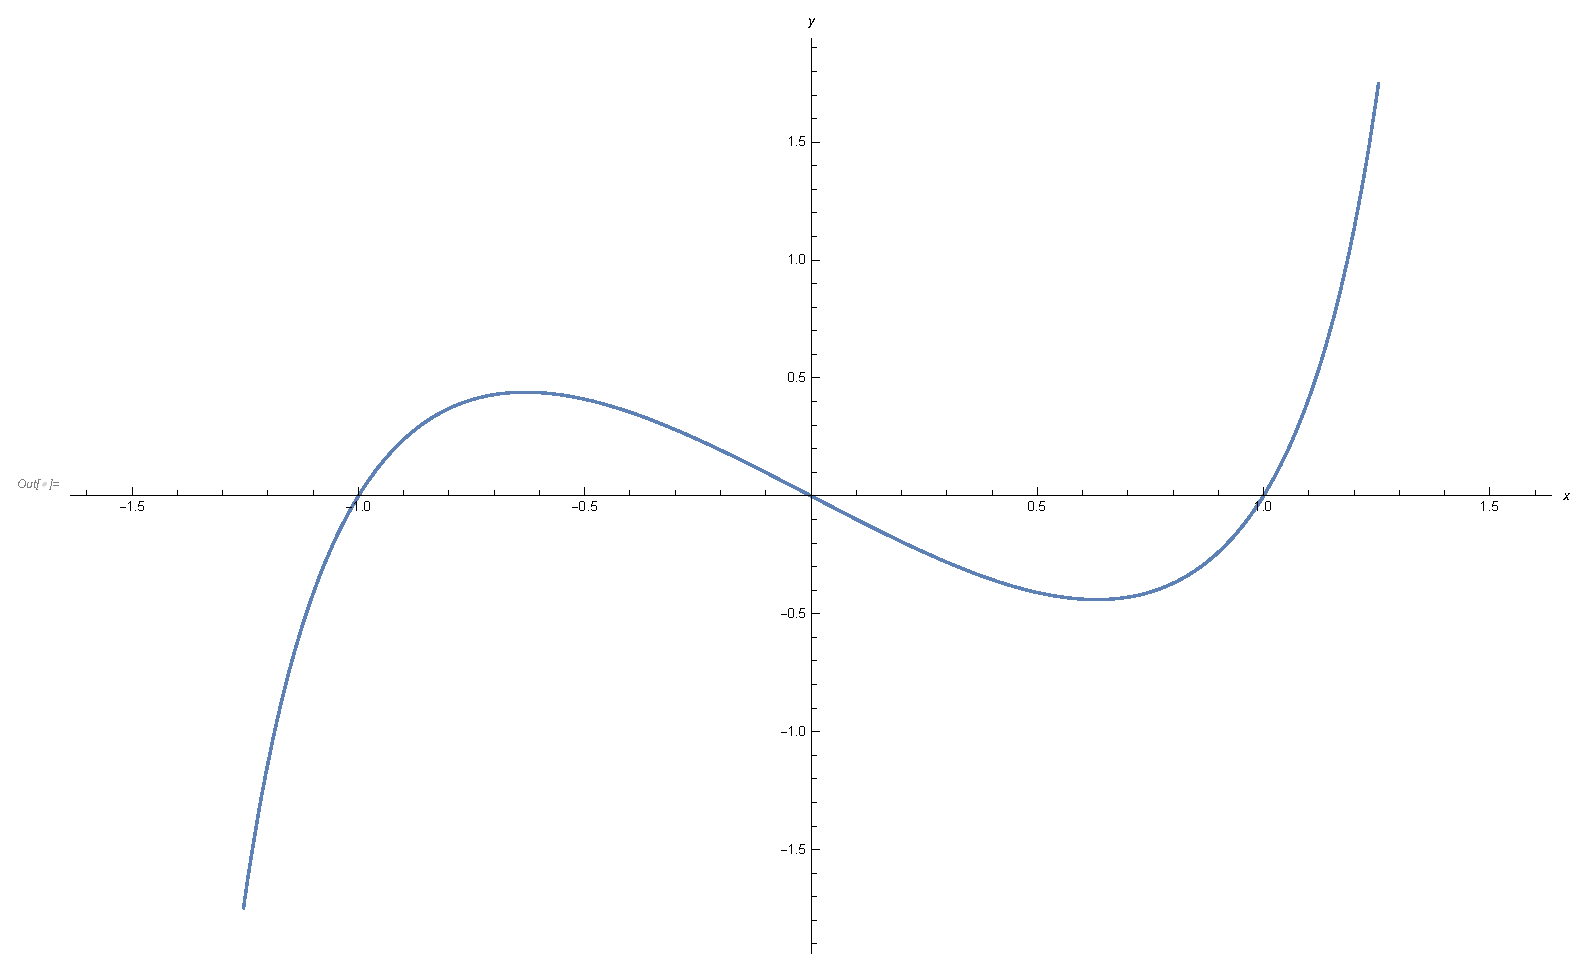
\includegraphics[width=0.9\textwidth]{curve_tracing_09_gr1.eps}

Roots

Mathematica will find the roots for us numerically.

\begin{doublespace}
\noindent\(\pmb{\text{FindRoot}[f[x],\{x,-1\}]}\)
\end{doublespace}

\begin{doublespace}
\noindent\(\{x\to -1.\}\)
\end{doublespace}

\begin{doublespace}
\noindent\(\pmb{\text{FindRoot}[f[x],\{x,0\}]}\)
\end{doublespace}

\begin{doublespace}
\noindent\(\{x\to 0.\}\)
\end{doublespace}

\begin{doublespace}
\noindent\(\pmb{\text{FindRoot}[f[x],\{x,1\}]}\)
\end{doublespace}

\begin{doublespace}
\noindent\(\{x\to 1.\}\)
\end{doublespace}

Therefore, the function f has three roots (intersections with the x axis). These are (-1, 0); (0, 0); and (1, 0).

\begin{doublespace}
\noindent\(\pmb{\text{Simplify}[f[x]=0]}\)
\end{doublespace}

\begin{doublespace}
\noindent\(0\)
\end{doublespace}

Setting the function f to zero, we get the intersection with the y axis which is at (0, 0).

Extreme Values

In this section, we want to find all maxima, minima and saddle points of the function f.

\section*{Derivatives}

Before we consider the extreme values for the function f, we want to find its derivatives. We have

\begin{doublespace}
\noindent\(\pmb{f'[x]}\)
\end{doublespace}

\begin{doublespace}
\noindent\(\pmb{\left(-1+x^2\right) \text{Sec}[x]^2+2 x \text{Tan}[x]}\)
\end{doublespace}

\begin{doublespace}
\noindent\(\pmb{\text{Plot}\left[f'[x],\left\{x,\frac{-\pi }{2},\frac{\pi }{2}\right\},\text{PlotStyle}\to \text{Orange}, \text{ImageSize}\to 1000\text{AxesLabel}\to
\{x,y\}\right]}\)
\end{doublespace}

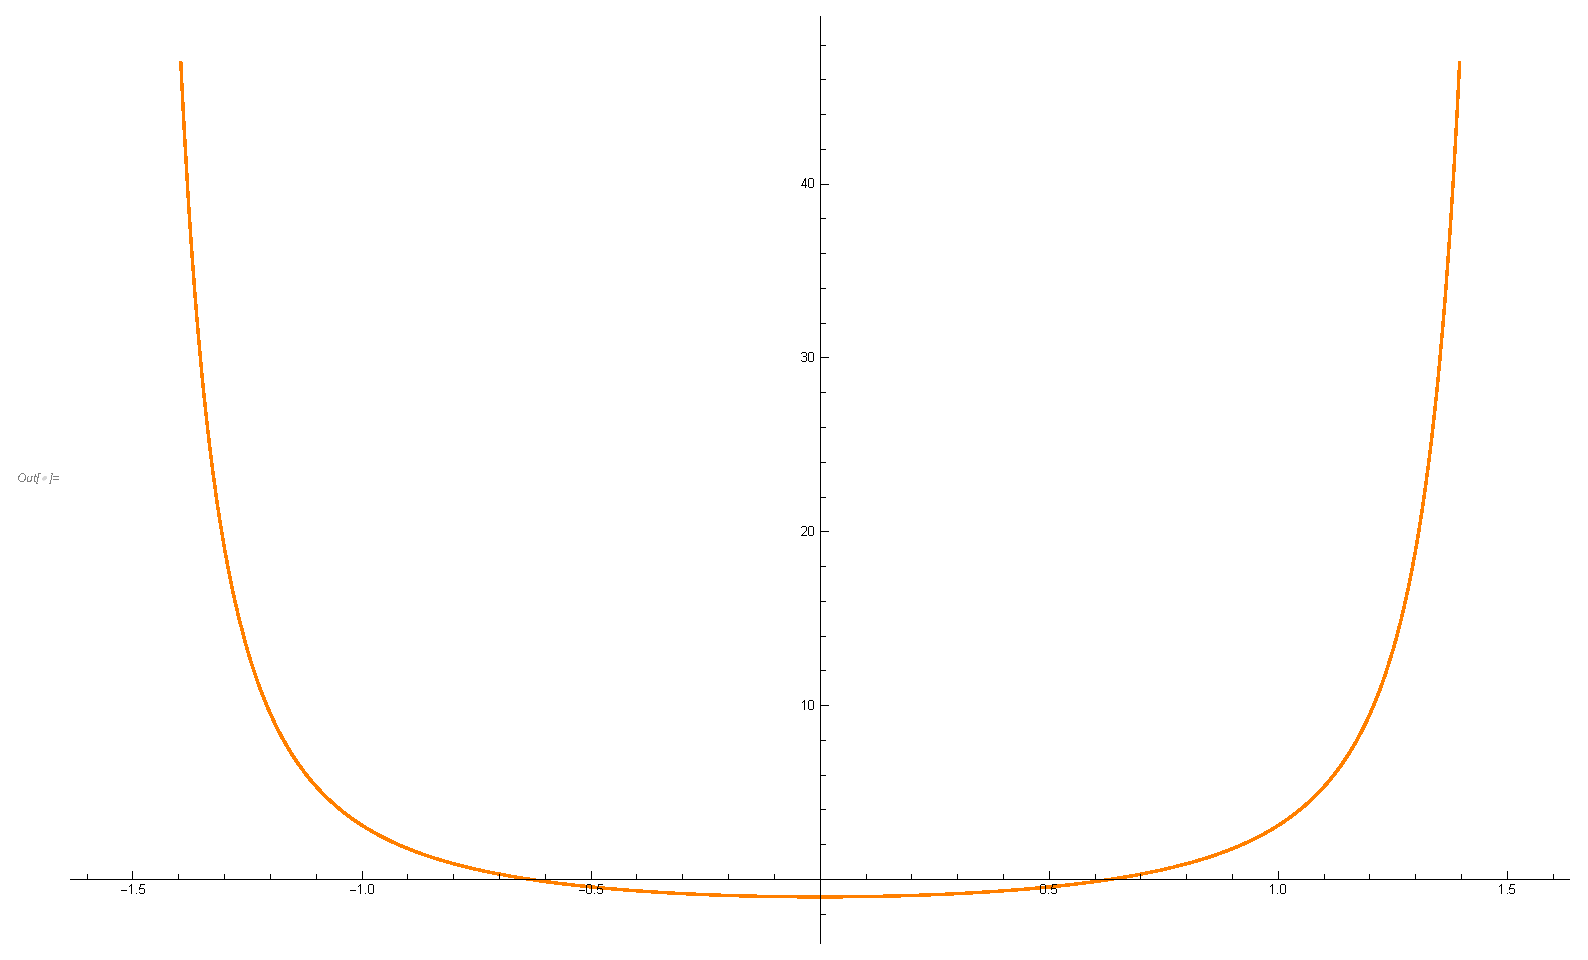
\includegraphics[width=0.9\textwidth]{curve_tracing_09_gr2.eps}

\begin{doublespace}
\noindent\(\pmb{f\text{''}[x]}\)
\end{doublespace}

\begin{doublespace}
\noindent\(4 x \text{Sec}[x]^2+2 \text{Tan}[x]+2 \left(-1+x^2\right) \text{Sec}[x]^2 \text{Tan}[x]\)
\end{doublespace}

\begin{doublespace}
\noindent\(\pmb{\text{Plot}\left[f\text{''}[x],\left\{x,\frac{-\pi }{2},\frac{\pi }{2}\right\}, \text{ImageSize}\to 1000,\text{PlotStyle}\to \text{Green}\right]}\)
\end{doublespace}

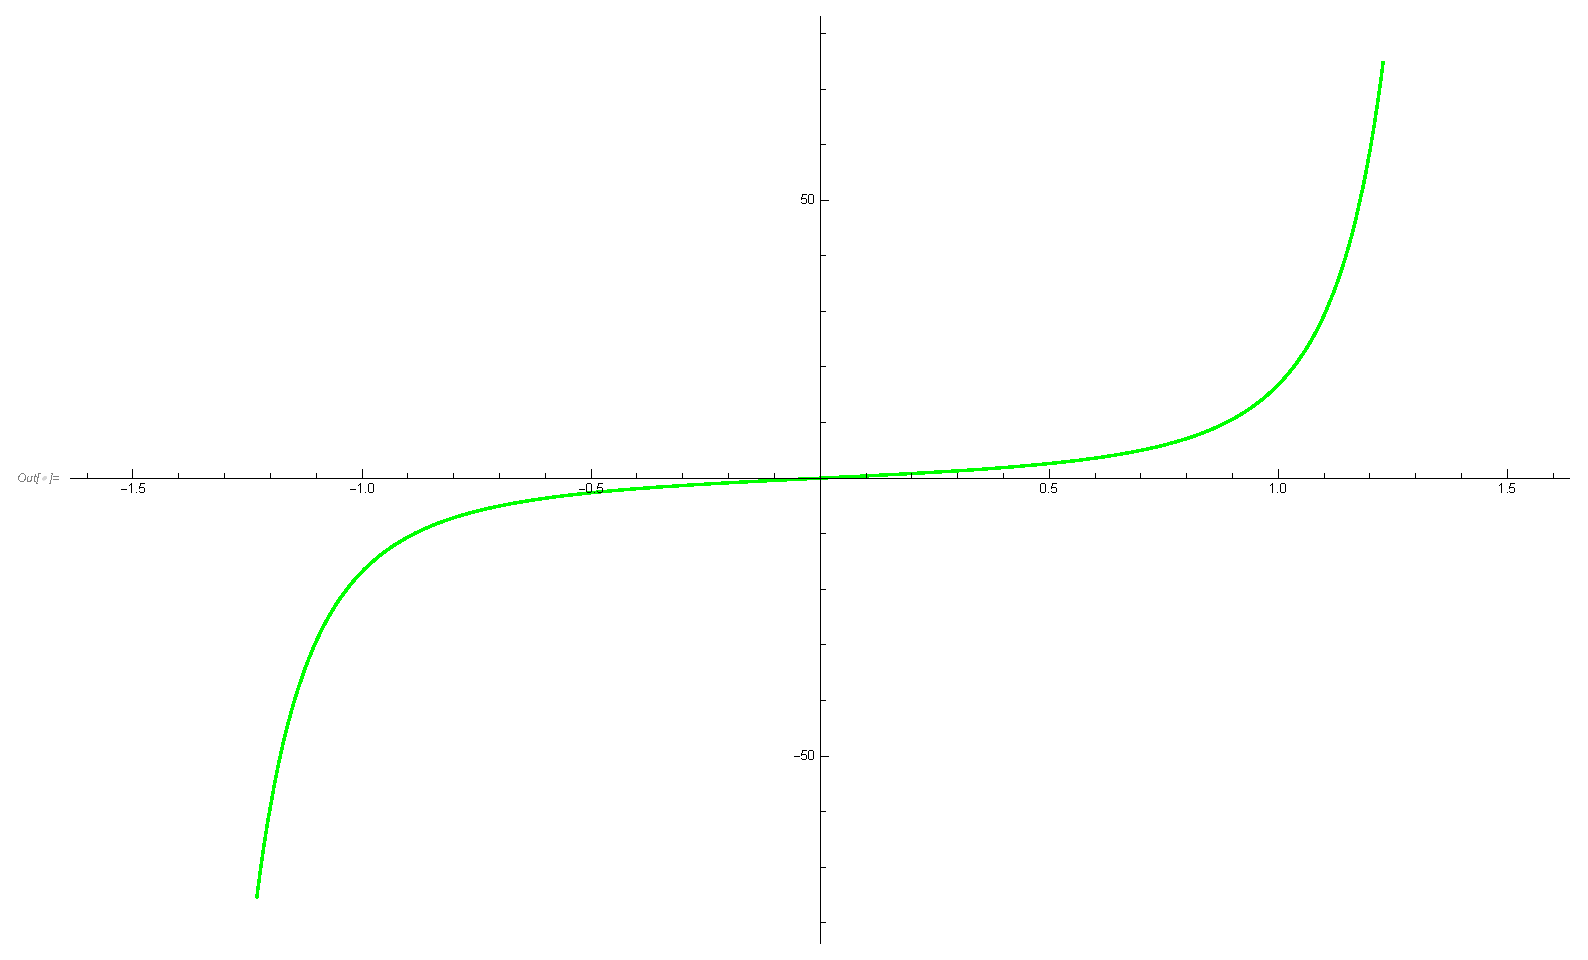
\includegraphics[width=0.9\textwidth]{curve_tracing_09_gr3.eps}

Putting the original function and its two derivatives in a plot, we get

\begin{doublespace}
\noindent\(\pmb{\text{Plot}\left[\left\{\left(x^2-1\right)\text{Tan}[x],f'[x],f\text{''}[x]\right\},\left\{x,\frac{-\pi }{2},\frac{\pi }{2}\right\},
\text{ImageSize}\to 1000,\text{PlotStyle}\to  \{\text{Dashed}, \text{Orange}, \text{Green}\},\text{PlotLegends}\to \text{{``}Expressions{''}}\right]}\)
\end{doublespace}

\begin{doublespace}
\noindent\(\begin{array}{cc}
  &  \\
\end{array}\)
\end{doublespace}

\section*{Extreme Values}

For the extreme values we have

\begin{doublespace}
\noindent\(\pmb{\text{FindMinimum}\left[\left(x^2-1\right)\text{Tan}[x],\{x,0.5\}\right]}\)
\end{doublespace}

\begin{doublespace}
\noindent\(\{-0.439732,\{x\to 0.631264\}\}\)
\end{doublespace}

\begin{doublespace}
\noindent\(\pmb{\text{FindMaximum}\left[\left(x^2-1\right)\text{Tan}[x],\{x,-0.5\}\right]}\)
\end{doublespace}

\begin{doublespace}
\noindent\(\{0.439732,\{x\to -0.631264\}\}\)
\end{doublespace}

To find saddle points we have

\begin{doublespace}
\noindent\(\pmb{\text{FindRoot}[f'[x],\{x,-1\}]}\)
\end{doublespace}

\begin{doublespace}
\noindent\(\{x\to -0.631264\}\)
\end{doublespace}

\begin{doublespace}
\noindent\(\pmb{\text{FindRoot}[f'[x],\{x,1\}]}\)
\end{doublespace}

\begin{doublespace}
\noindent\(\{x\to 0.631264\}\)
\end{doublespace}

These extreme values are already a minimum or a maximum; therefore, the function f does not have any saddle points.

Inflection Points

To find inflection points, we compute

\begin{doublespace}
\noindent\(\pmb{\text{FindRoot}[f\text{''}[x],\{x,0\}]}\)
\end{doublespace}

\begin{doublespace}
\noindent\(\{x\to 0.\}\)
\end{doublespace}

\begin{doublespace}
\noindent\(\pmb{f\text{''}[0]}\)
\end{doublespace}

\begin{doublespace}
\noindent\(0\)
\end{doublespace}

Therefore, the function f does not have any inflection points.

Singularity

The function f does not have a singularity in \(\left[\frac{-\pi }{2},\frac{\pi }{2}\right]\) since tan(x) = \(\frac{\sin (x)}{\cos (x)}\), but cos(x)
is never 0 for the given domain. In other words, the function f is defined everywhere on the given domain.

Limits

Since we do not have any singularity and the domain is a closed set, there is no limit to sensibly evaluate.

\end{document}
